\documentclass[]{spie}

\renewcommand{\baselinestretch}{1.0}
\usepackage{amsmath,amsfonts,amssymb}
\usepackage{graphicx}
\usepackage{cite}
\usepackage[T1]{fontenc}
\usepackage{times}
\usepackage[colorlinks=true,allcolors=blue]{hyperref}

\title{Benchmarking active spot selection for cost-efficient spatial transcriptomics}

\author[a]{Zheyu Zhu}
\author[b]{Junchao Zhu}
\author[c]{Fengbei Liu}
\author[b]{Tianyuan Yao}
\author[d]{Gelei Xu}
\author[e]{John Cannon}
\author[f]{Haichun Yang}
\author[b]{Yuankai Huo}
\author[c,g]{Mert R. Sabuncu}
\author[g]{Ruining Deng}

\affil[a]{University of Pennsylvania, Philadelphia, PA 19104, USA}
\affil[b]{Vanderbilt University, Nashville, TN, USA}
\affil[c]{Cornell Tech, New York, NY 10044, USA}
\affil[d]{University of Notre Dame, South Bend, IN 46556, USA}
\affil[e]{New York Medical College, Valhalla, NY 10595, USA}
\affil[f]{Vanderbilt University Medical Center, Nashville, TN 37232, USA}
\affil[g]{Weill Medical College of Cornell University, New York, NY 10065, USA}

\pagestyle{empty}

\authorinfo{Corresponding author: Ruining Deng\\
E-mail: rud4004@med.cornell.edu}

\begin{document}
\maketitle

\begin{abstract}
Can active learning (AL) select more useful spatial transcriptomics (ST) training spots than uniform Random sampling at the same label budget? We evaluate this question retrospectively on fully profiled HER2-positive breast cancer and cutaneous squamous cell carcinoma (cSCC) cohorts. Random, Monte Carlo dropout, temporal output discrepancy, CoreSet, and TypiClust-inspired selection share a DenseNet-121 predictor and six-round acquisition protocol. Four patient-level folds and budgets of 5\%, 10\%, 30\%, and 50\% give 160 budgeted configurations, each trained with one seed. Outcomes are within-slide gene-expression Pearson correlation (PCC), expression-cluster agreement, and Moran's~$I$ fidelity. All four active-strategy mean PCC differences are negative at 10\% on both cohorts. Averaging their differences from Random gives $-0.0176$ and $-0.0117$ at 5\% and 10\% on HER2, and $-0.0089$ and $-0.0087$ on cSCC. At 50\%, these differences are small and positive ($+0.0057$ and $+0.0028$). Higher expression-cluster agreement despite lower mean PCC occurs on HER2 but does not reproduce on cSCC. Target auditing identifies raw-log HER2 and library-scaled cSCC targets. We document physical image context, report paired fold effects, and add an exploratory correction for cross-validation dependence; no comparison survives multiplicity adjustment. These results provide no consistent low-budget PCC advantage for the tested active rules under this protocol. They do not establish equivalence to Random: seed variability, convergence, physical-scale harmonization, and prospective assay costs remain unresolved.
\end{abstract}

\keywords{spatial transcriptomics, active learning, spot selection, gene-expression prediction, benchmarking}

\section{Introduction}
\label{sec:intro}

\begin{figure}[htbp]
\centering
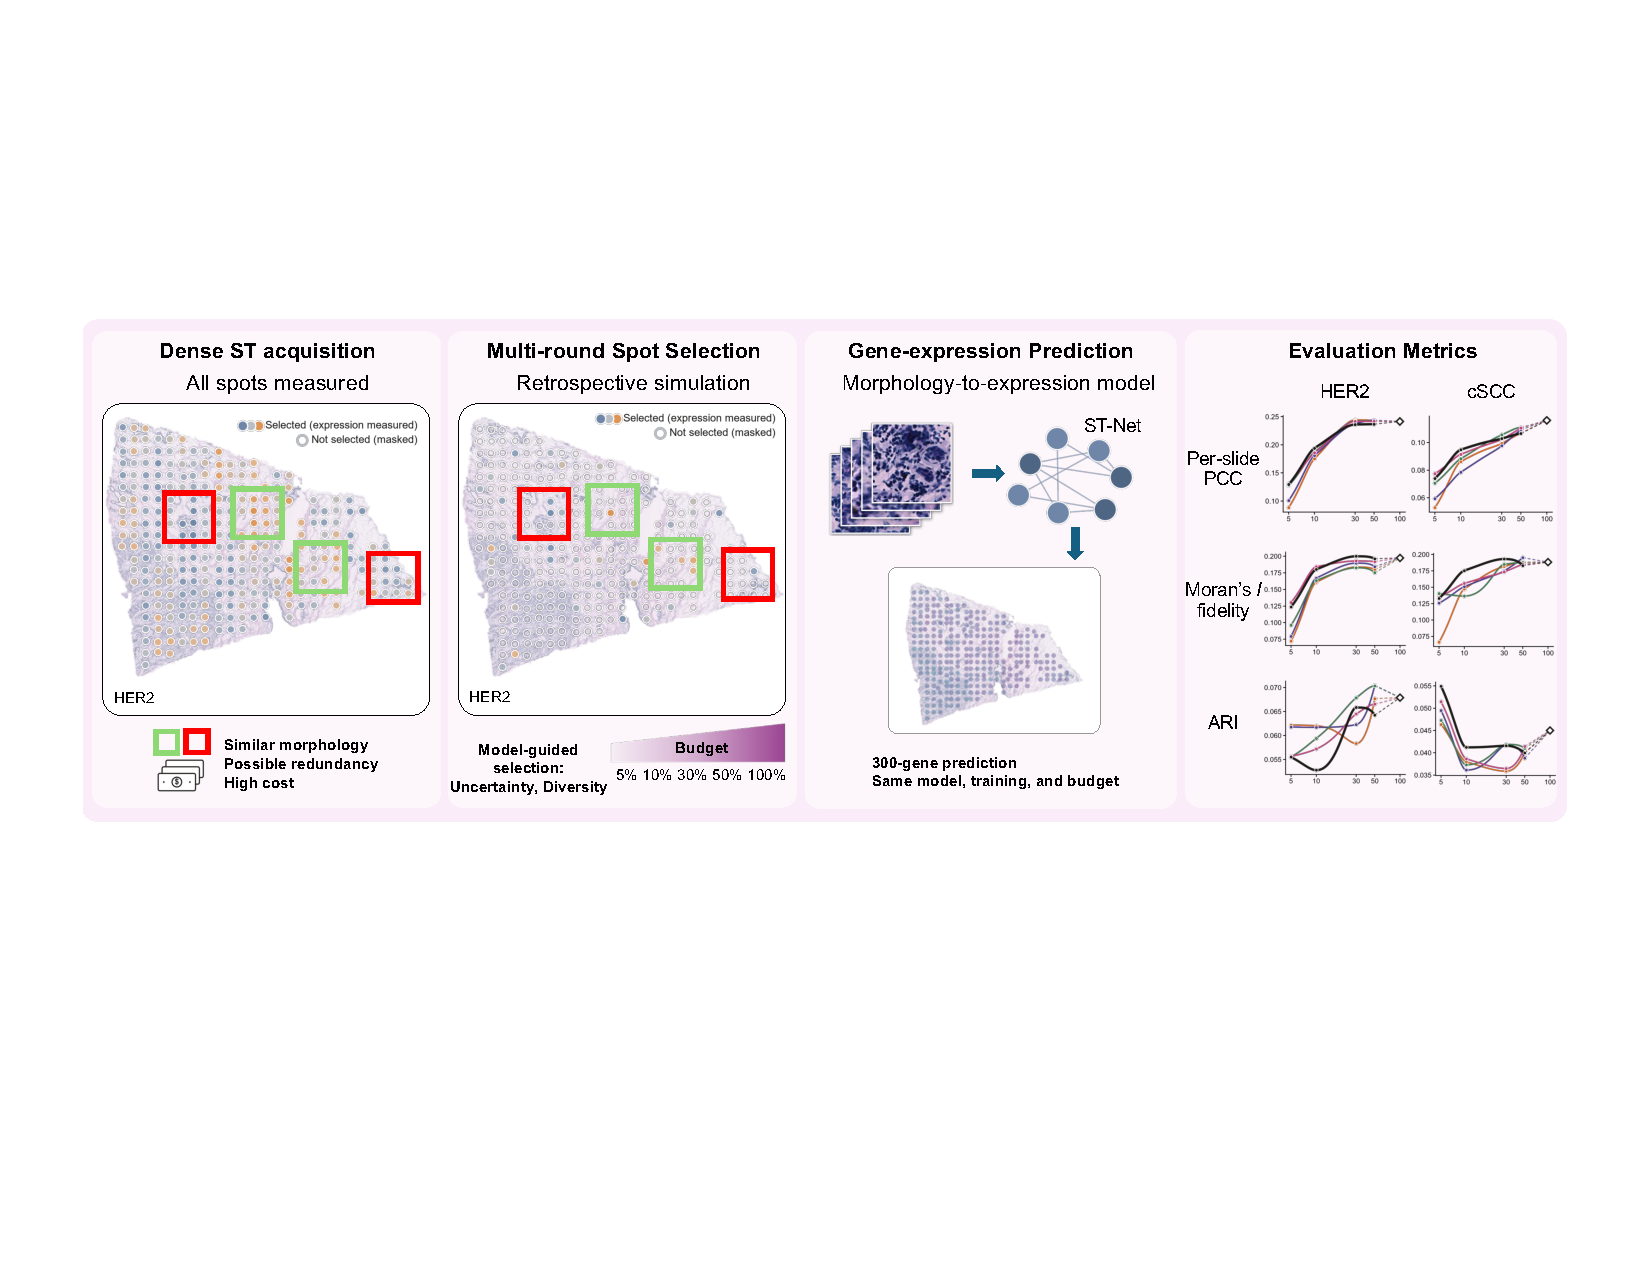
\includegraphics[width=\textwidth]{Figure/Image1.pdf}
\caption{Overview of the retrospective benchmark. H\&E images are available for all candidates; only expression labels are hidden and revealed for selected spots. The four budgets are separate experiments with budget-specific training horizons. The 100\% ticks and dashed connections mark the separate nominal full-label reference, not a fifth active-selection experiment or an optimization-matched upper bound. Outlined regions illustrate similar morphology without establishing expression redundancy. Curve colors are Random (black), CoreSet (orange), MC-dropout (purple), TOD (green), and TypiClust-inspired (magenta). Protocols are matched across strategies within a budget; stochastic training variation remains.}
\label{fig:overview}
\end{figure}

Spatial transcriptomics (ST) measures gene expression while preserving the spatial organization of tissue, supporting studies of tumor architecture, immune infiltration, and tissue development~\cite{stahl2016visualization,ji2020multimodal,andersson2021spatial,zhu2026comprehensive}. On commonly used barcoded-array platforms, tissue sections are profiled over a predefined grid of capture spots, including spots in morphologically similar regions. Because ST acquisition is substantially more expensive than routine whole-slide imaging~\cite{zhu2024asign}, dense acquisition can limit the number of patients and sections included in a study. Spatial gene expression can also be autocorrelated, so neighboring spots in histologically homogeneous regions may exhibit similar expression patterns. These properties motivate a practical question: can a selected subset of spots provide sufficient supervision for learning the relationship between tissue morphology and gene expression? Before customized capture regions or region-selective assays are developed, this premise can be tested retrospectively by comparing selected and uniformly sampled spot subsets of the same size.

Previous studies have developed many approaches for predicting spatial gene expression from hematoxylin and eosin (H\&E) images. ST-Net formulated patch-to-spot regression using a pretrained convolutional neural network~\cite{he2020integrating}; later methods incorporated spatial context through transformers and graph neural networks~\cite{pang2021leveraging,zeng2022spatial}, exemplar retrieval and contrastive learning~\cite{yang2023exemplar,xie2023bleep}, pathology foundation models~\cite{chen2024uni}, and other architectures~\cite{zhu2025magnet,zhu2025img2st,zhu2026duet}. SCR$^2$-ST instead considers efficient active sampling through reinforcement learning~\cite{zhu2025scr2}. The present study addresses a narrower benchmarking gap: under matched budgets and a shared predictor, how do standard uncertainty- and diversity-based acquisition strategies compare with Random sampling? This setting differs from conventional active learning (AL) because each spot has a high-dimensional continuous expression vector, neighboring candidates are spatially correlated, and a subset that improves pointwise expression prediction may not preserve spatial expression structure. AL performance can also depend on the available budget~\cite{hacohen2022active}, making evaluation at multiple budgets necessary.

Figure~\ref{fig:overview} summarizes our retrospective pool-based benchmark. Starting from two fully profiled public cohorts, we mask the expression vectors of training candidates and simulate multi-round selection. We compare Random sampling with Monte Carlo dropout (MC-dropout)~\cite{gal2016dropout,gal2017deep}, temporal output discrepancy (TOD)~\cite{huang2021semi}, CoreSet~\cite{sener2018active}, and a TypiClust-inspired strategy~\cite{hacohen2022active} at 5\%, 10\%, 30\%, and 50\% of the fold-wide training spot pool. All strategies use the same patient-level splits, selection schedule, morphology-to-expression predictor, and optimization protocol. We evaluate mean per-gene within-slide Pearson correlation coefficient (PCC), expression-cluster agreement, and Moran's~$I$ fidelity. The contribution is an empirical test of existing acquisition rules, not a new sampling algorithm. A negative result answers a bounded practical question: whether these implementations provide a consistent prediction gain that could justify their scoring cost in this setting. It does not establish that AL is ineffective in other tissues or that Random is statistically equivalent to active selection.

\section{Methods}
\label{sec:method}

\subsection{Retrospective Active Spot-Selection Benchmark}
\label{sec:benchmark}

We retrospectively simulate spot acquisition by masking expression labels in fully profiled ST cohorts. For a training fold with $N$ candidate spots, spot $i$ has an H\&E patch $x_i$ and a measured expression vector $y_i\in\mathbb{R}^{G}$, with $G=300$. Selecting a spot reveals its complete expression vector, so the budget counts spots rather than genes, reads, or image patches. The expression of unselected spots remains hidden throughout acquisition.

The candidate pool contains all training-fold spots pooled across patients and slides. A strategy can use candidate images and previously revealed expression but cannot access the expression of an unselected spot or data from a held-out patient. Because selection is global rather than slide-specific, the budget is a fraction of the fold-wide training pool and does not enforce equal coverage of each slide.

We evaluate $\beta\in\{0.05,0.10,0.30,0.50\}$ over $R=6$ acquisition rounds in one continuous training run. The first batch is selected by Random sampling because no task-adapted predictor is available. Within a fold and budget, strategies use the same quota, predictor, acquisition schedule, and training schedule. The per-round quota is $q=\lfloor\beta N/R\rfloor$, giving $Rq$ delivered spots. The predictor is not reinitialized between rounds, so later selections depend on the labeled set and preceding optimization. The nominal full-label reference ($\beta=1$) uses Random to release labels over the same six rounds, without informed scoring, and trains for 50 epochs. Integer quotas can leave up to five spots unused. It is contextual rather than an optimization-matched upper bound; we additionally compare its epoch-50 snapshot with the epoch-50 snapshot of Random at 50\%.

The benchmark evaluates individual training spots rather than prospective sequencing or contiguous capture regions. H\&E images are available for the entire pool; the experiment reduces revealed expression labels, not image acquisition. A spot fraction is a labeling-budget surrogate, not a measured reduction in reagent, read, or assay cost. The four active strategies use automated scores derived from model predictions or learned image features; they do not incorporate pathologist-defined morphology, tissue-compartment constraints, or clinical knowledge. Consequently, the benchmark tests the computational premise of automated spot selection but not expert-guided acquisition or the feasibility and biological performance of a region-selective assay.

\subsection{Acquisition Strategies}
\label{sec:strategies}

All strategies select without replacement from the fold-wide training pool and use deterministic image preprocessing during candidate scoring.

\noindent\textbf{Random.}
Random samples uniformly without replacement and is the reference baseline. Because sampling occurs over spots rather than slides, the expected number selected from a slide is proportional to its candidate count. Random requires neither model inference nor an acquisition-scoring pass.

\noindent\textbf{MC-dropout.}
MC-dropout~\cite{gal2016dropout,gal2017deep} estimates uncertainty using repeated stochastic forward passes with dropout enabled. Predictive variance is computed for each output gene and aggregated across the $G$ targets; candidates with the largest scores are selected. Batch-normalization layers remain in evaluation mode. Because expression targets are not standardized by gene, gene scale can influence the aggregate acquisition score.

\noindent\textbf{TOD.}
TOD~\cite{huang2021semi} scores candidate $i$ by temporal prediction change:
\begin{equation}
s_{\mathrm{TOD}}(i)=\left\|f_{\theta_t}(x_i)-f_{\theta_{t-1}}(x_i)\right\|_2.
\label{eq:tod}
\end{equation}
As shown in Eq.~\ref{eq:tod}, a large score indicates that a candidate's predicted expression vector changes substantially between two model states. Predictions are cached by spot identifier. When no preceding cache is available, TOD uses Random selection. This implementation adapts the score to 300-output regression.

\noindent\textbf{CoreSet.}
CoreSet~\cite{sener2018active} applies greedy $k$-center selection to learned image features. Previously labeled features are the initial centers, and each step adds the candidate farthest from its nearest center under Euclidean distance. Features are extracted immediately before the regression head and are not $L_2$-normalized. CoreSet therefore measures feature-space coverage, not physical-space coverage.

\noindent\textbf{TypiClust-inspired.}
The TypiClust-inspired strategy~\cite{hacohen2022active} clusters current candidate features and selects a typical member of each cluster using within-cluster neighbor distance. Unlike the published method, this implementation uses task-predictor rather than self-supervised features and sets the cluster count to the round quota instead of $\min(|\mathcal{L}|+B,K_{\max})$. Its first round uses Random sampling because task-adapted features are initially unavailable.

Numerical strategy settings and acquisition timing are reported in Section~\ref{sec:setup}.

\subsection{Shared Morphology-to-Expression Predictor}
\label{sec:predictor}

All strategies use the same ST-Net-style predictor~\cite{he2020integrating}: a DenseNet-121 trunk~\cite{huang2017densely}, global average pooling, a 1,024-unit linear layer, a rectified linear unit, dropout, and a $G$-output regression layer. The trunk is initialized with torchvision's \texttt{IMAGENET1K\_}\allowbreak\texttt{V1} weights. All parameters are trainable, and mean squared error is applied to the targets defined in Section~\ref{sec:setup}. Using one predictor controls the architecture within this benchmark; it does not establish that the acquisition rankings transfer to other backbones or objectives.

\section{Data and Experimental Design}
\label{sec:data}

\subsection{Datasets and Experimental Setup}
\label{sec:setup}

We use two public legacy Spatial Transcriptomics cohorts from HEST-1k~\cite{jaume2024hest}: HER2-positive breast cancer~\cite{andersson2021spatial} and cutaneous squamous cell carcinoma (cSCC)~\cite{ji2020multimodal} (Table~\ref{tab:datasets}).

\begin{table}[htbp]
\centering
\caption{Cohorts used in the conference benchmark. Counts reflect HEST-1k preprocessing.}
\label{tab:datasets}
\resizebox{0.8\textwidth}{!}{%
\begin{tabular}{lccccc}
\hline
Cohort & Patients & Slides & Spots & Retained genes & Targets \\
\hline
HER2-positive breast cancer & 8 & 36 & 13,620 & 967 & 300 \\
cSCC & 4 & 12 & 8,671 & 392 & 300 \\
\hline
\end{tabular}
}
\end{table}

Cross-validation is patient-level. Each of four HER2-positive folds holds out two patients (9 slides; 2,457--3,810 spots), and each cSCC fold holds out one patient (3 slides; 1,632--3,398 spots). Held-out patients are used only for final evaluation.

Each input is a centered $224\times224$-pixel H\&E patch. The trainer consumes the supplied \texttt{expression\_norm} vectors without further normalization, using the first $G=300$ alphabetically ordered retained genes. A direct audit against barcode-aligned HEST raw counts found different target construction across cohorts:
\begin{equation}
\tilde y_{ig}=\begin{cases}
\log(1+c_{ig}), & \text{HER2},\\[2pt]
\log\!\left(1+10^4 c_{ig}/L_i\right), & \text{cSCC},
\end{cases}\qquad
L_i=\sum_{h\in\mathcal J}c_{ih}.
\label{eq:targets}
\end{equation}
Here $\mathcal J$ is the intersection of the raw HEST gene names across the 12 cSCC slides ($|\mathcal J|=13{,}251$), not the 392 retained genes in Table~\ref{tab:datasets} or the 300-output panel. The cSCC transformation was reconstructed empirically: it matches all $8{,}671\times300$ target values to within $2.4\times10^{-7}$; HER2 raw-log targets match exactly. Saved ground truth from the Random-50\% runs equals the supplied target vectors on all 48 slides. The original target-producing script was not recovered, so this numerical reconstruction documents the consumed targets rather than claiming a fully traced preprocessing history. Neither cohort's outputs are gene-wise standardized. These preprocessing differences limit cross-cohort interpretation even though all strategies within a cohort use identical targets.

Five sampling strategies, four budgets, and four folds give 80 completed configurations per cohort and 160 in total; full-label references are separate. Acquisition occurs at epochs 0, 5, 8, 11, 14, and 17 before gradient updates. TOD uses Random at epoch 5 because no preceding cache exists and therefore controls four rounds; the other active strategies control five. With $q=\lfloor\beta N/R\rfloor$, delivered totals can be up to $R-1$ spots below nominal (Table~\ref{tab:protocol}).

\begin{table}[htbp]
\centering
\caption{Budget and training settings for HER2-positive breast cancer fold 1, with $N=9{,}810$ training spots and $R=6$ acquisition rounds.}
\label{tab:protocol}
\begin{tabular}{lccccc}
\hline
$\beta$ & Nominal & Delivered & Per round & Epochs & Optimizer steps \\
\hline
0.05 & 490 & 486 & 81 & 110 & 715 \\
0.10 & 981 & 978 & 163 & 80 & 930 \\
0.30 & 2,943 & 2,940 & 490 & 70 & 2,260 \\
0.50 & 4,905 & 4,902 & 817 & 60 & 3,156 \\
\hline
\end{tabular}
\end{table}

Training uses stochastic gradient descent with momentum 0.9, no Nesterov acceleration, weight decay $10^{-4}$, and batch size 80 with the final partial batch retained. The learning rate is
\begin{equation}
\eta(u)=10^{-4}\left(1-\frac{u}{10^{8}}\right)^{0.9},
\label{eq:lr}
\end{equation}
where $u$ is the cumulative optimizer-update index and $10^{8}$ is the configured maximum-iteration denominator, not the epoch horizon. The rate is therefore nearly constant over these runs. Equation~\ref{eq:lr} runs continuously as the labeled set grows; final-epoch predictions are evaluated. Training applies horizontal and vertical flips independently ($p=0.5$ each), followed by a $90^{\circ}$ rotation ($p=0.5$); scoring is deterministic, without stain normalization or color augmentation. MC-dropout uses five passes with head dropout $p=0.3$ and batch normalization in evaluation mode. TypiClust-inspired uses $k$-means with $n_{\mathrm{init}}=3$ and at most 20 within-cluster neighbors.

All configurations use seed 42 and one NVIDIA RTX 3080 (10~GB) with Python 3.11.15, PyTorch 2.6.0, torchvision 0.21.0, CUDA 12.4, cuDNN 9.1.0, and scikit-learn 1.9.0. Deterministic algorithms are disabled and training randomness is not paired across strategies. Optimizer exposure also increases with budget (715 versus 3,156 steps at 5\% and 50\% in Table~\ref{tab:protocol}); cross-budget comparisons therefore reflect the stated training horizons, not matched optimization or convergence.

\subsection{Image Resolution and Physical Context}
\label{sec:resolution}

We distinguish H\&E image sampling scale from the ST capture grid's spatial resolution. A fixed pixel width does not imply a fixed physical field of view: a 224-pixel patch spans $224m$ micrometers per side at scale $m$ micrometers/pixel (Table~\ref{tab:resolution}). Training uses the pre-extracted PNG patches, not HEST's separately downsampled HDF5 patch images. Header checks on all 22,291 referenced PNGs confirmed $224\times224$ pixels. Twelve sampled patches from four locally available HER2 whole-slide images exactly matched native-resolution crops. cSCC scale relies on the corresponding slide metadata; local cSCC whole-slide images were unavailable for independent pixel matching. The training transform's resize to $224\times224$ is therefore not physical-scale harmonization.

\begin{table}[htbp]
\centering
\caption{Observed H\&E scale and physical patch context. These are image scales, not capture-spot diameters or evidence of single-cell resolution. Ranges are computed from slide metadata for the actual training cohort.}
\label{tab:resolution}
\begin{tabular}{lccc}
\hline
Cohort & Slides & H\&E scale ($\mu$m/pixel) & Patch width ($\mu$m) \\
\hline
HER2-positive breast cancer & 36 & 0.662--0.946 & 148.3--212.0 \\
cSCC & 12 & 0.545--0.554 & 122.2--124.1 \\
\hline
\end{tabular}
\end{table}

Within each paired strategy comparison, candidates and their physical image scale are identical. This controls scale as an input difference between arms but does not establish that strategy rankings are invariant to scale. Image scale was not randomized, and patient and acquisition characteristics are confounded. We did not retrain after matching physical context or assess multiple ST capture resolutions. The available images therefore support a scale audit, not a causal estimate of the effect of resolution.

\subsection{Evaluation and Reporting}
\label{sec:evaluation}

\noindent\textbf{Gene-expression accuracy.}
Within each held-out slide, PCC is computed across spots per gene and averaged over genes, then aggregated within the fold. Correlations are averaged without Fisher transformation; a $10^{-8}$ denominator stabilizer makes constant genes contribute approximately zero.

\noindent\textbf{Expression-cluster agreement.}
Predicted and measured profiles are clustered independently within each slide using $k$-means ($k=10$, $n_{\mathrm{init}}=10$, seed 42) without scaling or dimensionality reduction. Adjusted Rand index (ARI)~\cite{hubert1985comparing} compares the partitions; slides with fewer than $2k$ spots are excluded. This measures expression-cluster agreement, not histological domain recovery.

\noindent\textbf{Moran's $I$ fidelity.}
Moran's $I$~\cite{moran1950notes} is computed per slide and gene using a symmetrized six-nearest-neighbor graph on array coordinates with binary, non-row-standardized weights. Fidelity is the PCC across genes between measured and predicted Moran's $I$; at least three defined genes are required.

\noindent\textbf{Statistical reporting.}
The unit of comparison is a paired held-out fold, not a spot or gene. We report fold means and sample SDs, active-minus-Random differences, and positive-fold counts. Pooling four strategies gives a descriptive average with a shared Random comparator, not 16 independent observations. Each method--budget--fold configuration has one seed, including Random; fold SD is not uncertainty across training or acquisition seeds.

As an exploratory sensitivity analysis, we apply the corrected cross-validation $t$ statistic~\cite{bouckaert2004replicability}: for four paired differences with mean $\bar d$ and sample variance $s_d^2$, $\mathrm{SE}_{\mathrm{corr}}=\sqrt{(1/4+1/3)s_d^2}$ and $t=\bar d/\mathrm{SE}_{\mathrm{corr}}$ with three degrees of freedom. The $1/3$ term is the nominal held-out-to-training patient ratio. We report pointwise approximate 95\% intervals and apply Holm adjustment~\cite{holm1979simple} across all 32 PCC comparisons (two cohorts, four active rules, four budgets), using a two-sided 0.05 threshold. This heuristic correction acknowledges overlapping training folds but is not calibrated for this small, heterogeneous, grouped-regression dataset. It cannot estimate seed variability or establish equivalence. ARI, Moran fidelity, pooled strategy averages, and the epoch-50 comparison remain descriptive.

\noindent\textbf{Acquisition cost.}
Acquisition cost is per-round candidate-scoring time, including required feature extraction but excluding training. Random has no scoring pass. We summarize available rounds by their within-fold median, then report the range across folds. These are logged timings rather than independent repeated timing trials under monitored machine load. The later TypiClust-inspired sessions and an earlier timing outlier are distinguished explicitly; timings do not establish platform-independent complexity or assay cost.

\section{Results}
\label{sec:results}

\subsection{Gene-Expression Accuracy Across Budgets}

PCC generally increases with budget on both cohorts (Tables~\ref{tab:pcc_her2} and~\ref{tab:pcc_cscc}), but between-fold variation exceeds the mean differences among strategies. To quantify training-horizon sensitivity, let $r=100(\bar p_E-\bar p_{E-10})/\bar p_E$, using the four-fold mean PCC at final epoch $E$ and ten epochs earlier. Across strategies and cohorts, $r$ ranges from $+10.1$\% to $+27.8$\% at 5\%, $+4.6$\% to $+23.0$\% at 10\%, $-3.3$\% to $+3.5$\% at 30\%, and $-2.0$\% to $+4.0$\% at 50\%. Thus the low-budget models remain sensitive to training duration, and even the high-budget tail does not prove convergence. Comparisons apply to the stated horizons, not independently optimized predictors.

The nominal full-label reference reaches $0.2416\pm0.1460$ on HER2-positive breast cancer and $0.1160\pm0.0220$ on cSCC. Random at 5\% reaches 54\% and 64\% of these means, and Random at 50\% reaches 98\% and 92\%, respectively. These ratios neither establish noninferiority nor quantify sequencing-cost savings: PCC is not a linear measure of recovered biological signal, and the reference uses 50 epochs versus 60 at 50\%.

At a common elapsed epoch of 50, the full-label-minus-Random-50\% difference is $+0.0058$ on HER2 (positive in 3/4 folds) and $+0.0073$ on cSCC (4/4). This checks the sensitivity of the reference comparison to elapsed training duration. It does not equalize optimizer exposure: the full-label reference receives 5,028--5,721 updates on HER2 and 2,695--3,600 on cSCC, versus 2,536--2,865 and 1,353--1,804 for the 50\% arm. A larger labeled set changes the number of updates per epoch, so no optimization-matched upper-bound claim follows.

\begin{table}[htbp]
\centering
\caption{HER2-positive breast cancer PCC, mean $\pm$ sample SD over four folds. Bold marks the largest mean per budget; cost is the range of logged fold-median scoring times at 50\%. TypiClust-inspired uses three later-session folds; its earlier 1,584-second fold-median outlier is reported separately in the text.}
\label{tab:pcc_her2}
\resizebox{\textwidth}{!}{%
\begin{tabular}{lccccr}
\hline
Strategy & 5\% & 10\% & 30\% & 50\% & Cost/round \\
\hline
Random & $0.1295 \pm 0.0682$ & $\mathbf{0.1940} \pm 0.1042$ & $0.2361 \pm 0.1342$ & $0.2367 \pm 0.1375$ & $<1$\,s \\
CoreSet~\cite{sener2018active} & $0.0883 \pm 0.0495$ & $0.1751 \pm 0.0998$ & $\mathbf{0.2442} \pm 0.1297$ & $0.2422 \pm 0.1396$ & $11$--$12$\,s \\
MC-dropout~\cite{gal2016dropout} & $0.1009 \pm 0.0582$ & $0.1811 \pm 0.1013$ & $0.2378 \pm 0.1298$ & $\mathbf{0.2439} \pm 0.1398$ & $37$--$42$\,s \\
TOD~\cite{huang2021semi} & $0.1276 \pm 0.0873$ & $0.1870 \pm 0.1109$ & $0.2428 \pm 0.1355$ & $0.2418 \pm 0.1427$ & $7$--$8$\,s \\
TypiClust-inspired~\cite{hacohen2022active} & $\mathbf{0.1308} \pm 0.0701$ & $0.1857 \pm 0.0994$ & $0.2418 \pm 0.1352$ & $0.2417 \pm 0.1450$ & $71$--$83$\,s \\
\hline
\multicolumn{6}{l}{\emph{Nominal full-label reference (}$\beta=1$\emph{, 50 epochs): $0.2416 \pm 0.1460$}} \\
\hline
\end{tabular}
}
\end{table}

\begin{figure}[htbp]
\centering
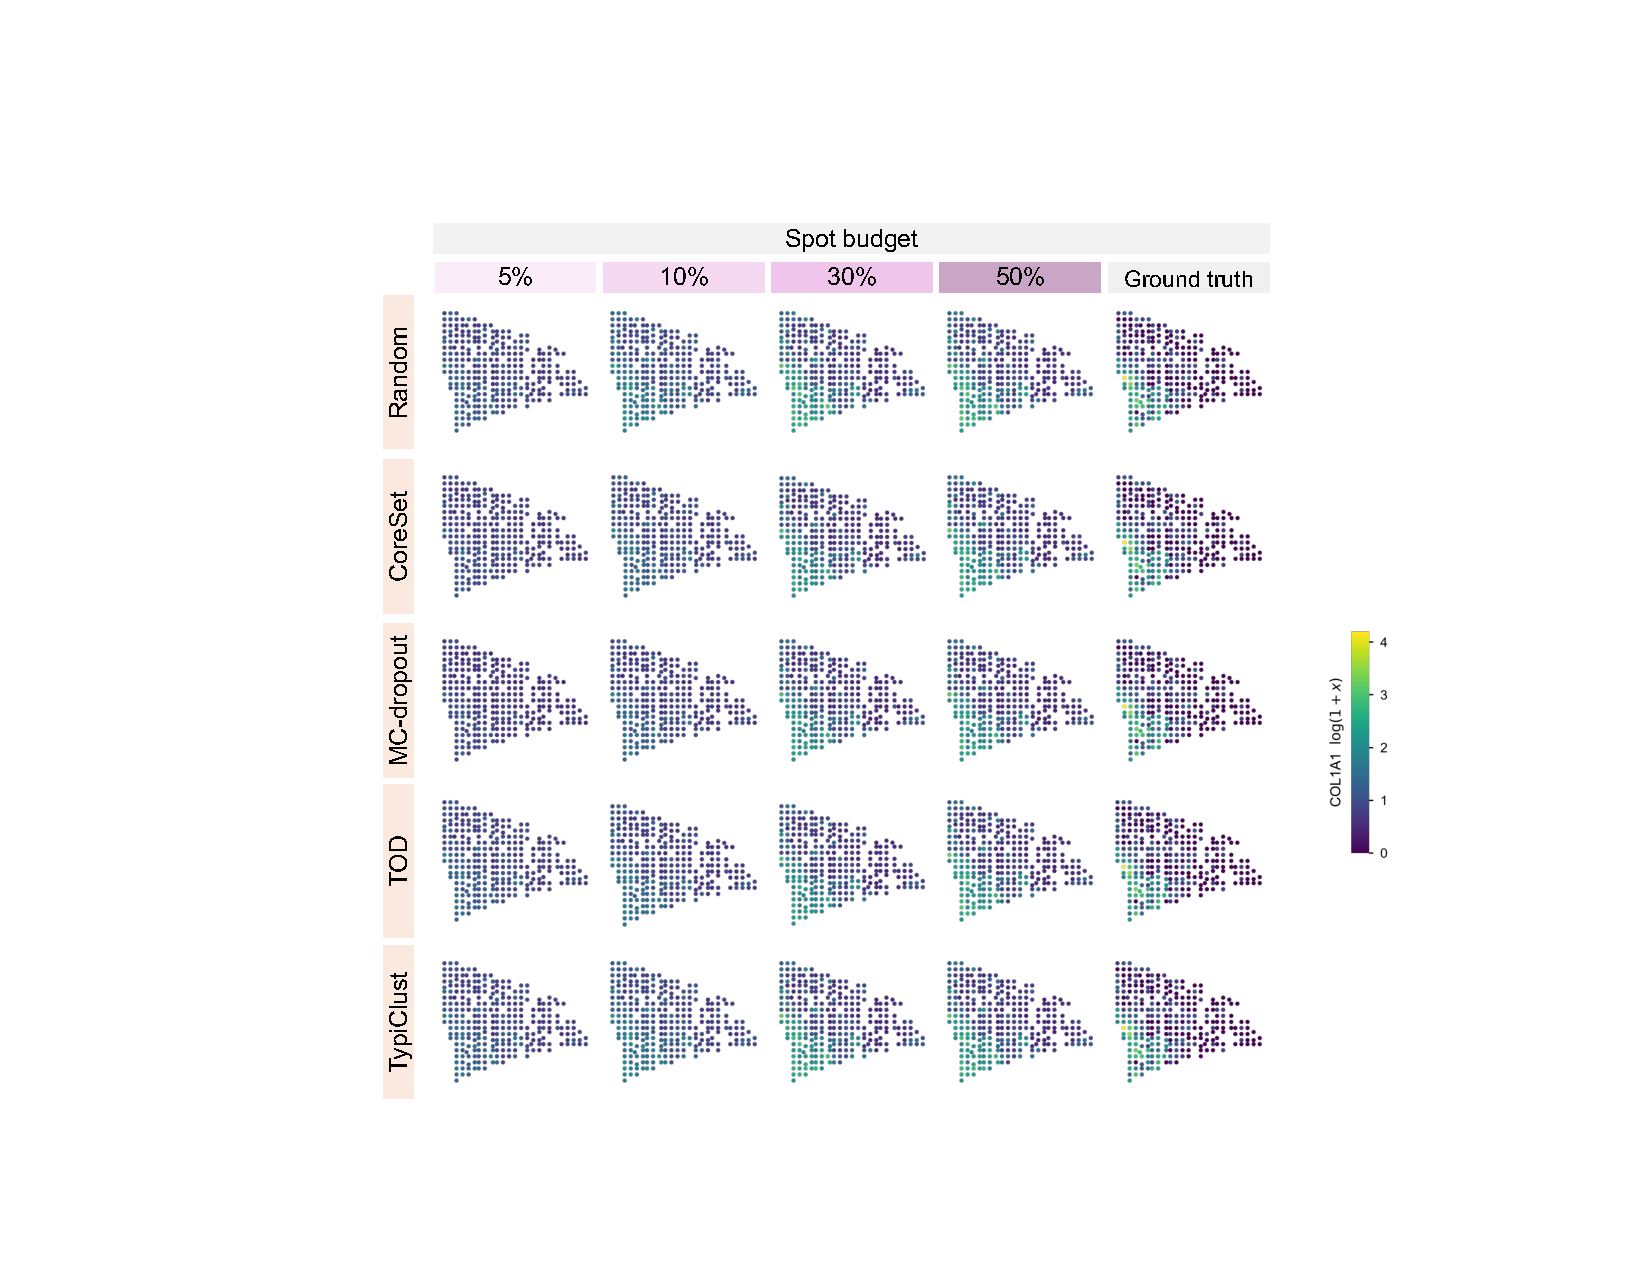
\includegraphics[width=\textwidth]{Figure/Image2.pdf}
\caption{Predicted \textit{COL1A1} on held-out HER2-positive slide SPA143. Rows are strategies, columns are budgets, and all panels share the measured-map scale. Predicted SD increases from 0.18--0.28 at 5\% to 0.67--0.70 at 50\%, versus 0.87 measured. This single-slide example is not used to rank strategies.}
\label{fig:predmaps}
\end{figure}

\subsection{Paired Comparison With Random}

On both cohorts, three active-strategy means are below Random at 5\% and all four are below Random at 10\%. At 30\%, all four mean differences are positive on HER2, whereas three remain negative on cSCC; at 50\%, all four are slightly positive on both cohorts (Table~\ref{tab:paired}). Averaged descriptively across strategies, the cSCC differences are $-0.0089$, $-0.0087$, $-0.0016$, and $+0.0028$. Thus there is no common 30\% crossover across these cohorts.

None of the 32 exploratory corrected PCC tests reaches the two-sided 0.05 threshold, before or after Holm adjustment (minimum unadjusted $p=0.128$; all adjusted $p=1.000$). For example, HER2 CoreSet at 5\% has a mean difference of $-0.0412$ and no positive folds, but its approximate corrected 95\% interval is $[-0.1041,\,0.0216]$. The interval illustrates the limited precision of four overlapping folds. These tests do not establish a zero effect, reproducibility across seeds, or equivalence to Random. The bounded empirical finding is the repeated direction of the low-budget cohort means under the specified protocol.

\begin{table}[htbp]
\centering
\caption{Paired PCC difference from Random; parentheses give positive folds out of four. Pooled rows are descriptive because strategies share the Random comparator.}
\label{tab:paired}
\begin{tabular}{lcccc}
\hline
Strategy & 5\% & 10\% & 30\% & 50\% \\
\hline
\multicolumn{5}{l}{\emph{HER2-positive breast cancer}} \\
CoreSet~\cite{sener2018active} & $-0.0412$ (0/4) & $-0.0189$ (1/4) & $+0.0081$ (2/4) & $+0.0055$ (4/4) \\
MC-dropout~\cite{gal2016dropout} & $-0.0286$ (1/4) & $-0.0129$ (1/4) & $+0.0017$ (1/4) & $+0.0072$ (3/4) \\
TOD~\cite{huang2021semi} & $-0.0019$ (2/4) & $-0.0069$ (2/4) & $+0.0067$ (3/4) & $+0.0051$ (3/4) \\
TypiClust-inspired~\cite{hacohen2022active} & $+0.0013$ (2/4) & $-0.0082$ (0/4) & $+0.0057$ (4/4) & $+0.0050$ (2/4) \\
Pooled mean $\Delta$ & $-0.0176$ & $-0.0117$ & $+0.0055$ & $+0.0057$ \\
Pooled positive & 5/16 & 4/16 & 10/16 & 12/16 \\
\hline
\multicolumn{5}{l}{\emph{cSCC}} \\
CoreSet~\cite{sener2018active} & $-0.0212$ (1/4) & $-0.0086$ (1/4) & $-0.0035$ (2/4) & $+0.0002$ (2/4) \\
MC-dropout~\cite{gal2016dropout} & $-0.0146$ (1/4) & $-0.0163$ (0/4) & $-0.0052$ (2/4) & $+0.0027$ (3/4) \\
TOD~\cite{huang2021semi} & $-0.0034$ (2/4) & $-0.0065$ (2/4) & $+0.0027$ (3/4) & $+0.0043$ (4/4) \\
TypiClust-inspired~\cite{hacohen2022active} & $+0.0034$ (3/4) & $-0.0034$ (1/4) & $-0.0005$ (1/4) & $+0.0040$ (4/4) \\
Pooled mean $\Delta$ & $-0.0089$ & $-0.0087$ & $-0.0016$ & $+0.0028$ \\
Pooled positive & 7/16 & 4/16 & 8/16 & 13/16 \\
\hline
\end{tabular}
\end{table}

\begin{table}[htbp]
\centering
\caption{cSCC PCC, mean $\pm$ SD over four folds. Bold marks the largest mean per budget.}
\label{tab:pcc_cscc}
\resizebox{0.95\textwidth}{!}{%
\begin{tabular}{lcccc}
\hline
Strategy & 5\% & 10\% & 30\% & 50\% \\
\hline
Random & $0.0740 \pm 0.0253$ & $\mathbf{0.0948} \pm 0.0233$ & $0.1029 \pm 0.0212$ & $0.1066 \pm 0.0209$ \\
CoreSet~\cite{sener2018active} & $0.0528 \pm 0.0260$ & $0.0862 \pm 0.0233$ & $0.0994 \pm 0.0130$ & $0.1068 \pm 0.0169$ \\
MC-dropout~\cite{gal2016dropout} & $0.0594 \pm 0.0266$ & $0.0785 \pm 0.0192$ & $0.0977 \pm 0.0181$ & $0.1093 \pm 0.0228$ \\
TOD~\cite{huang2021semi} & $0.0705 \pm 0.0193$ & $0.0883 \pm 0.0173$ & $\mathbf{0.1056} \pm 0.0215$ & $\mathbf{0.1109} \pm 0.0214$ \\
TypiClust-inspired~\cite{hacohen2022active} & $\mathbf{0.0774} \pm 0.0270$ & $0.0915 \pm 0.0230$ & $0.1024 \pm 0.0229$ & $0.1106 \pm 0.0215$ \\
\hline
\multicolumn{5}{l}{\emph{Nominal full-label reference (}$\beta=1$\emph{, 50 epochs): $0.1160 \pm 0.0220$}} \\
\hline
\end{tabular}
}
\end{table}

\subsection{Spatial-Expression Structure}

At 5\% and 10\% on HER2-positive breast cancer, CoreSet and MC-dropout have lower mean PCC but higher ARI than Random; their ARI differences are positive on all four folds, whereas PCC has positive-fold exceptions (Tables~\ref{tab:paired} and~\ref{tab:spatial}). Figure~\ref{fig:predmaps} is an illustrative single-slide example, not independent validation. This reversal does not reproduce on cSCC, where every active-strategy mean ARI is below Random at both budgets (Table~\ref{tab:spatial_cscc}). Moran's $I$ fidelity also has no consistently best active strategy: TypiClust-inspired has the highest HER2 mean at 5\% and 10\%, Random at 30\% and 50\%, and the cSCC leader varies with budget. These expression-derived spatial measures do not establish histological-domain or biological-pathway recovery.

\begin{table}[htbp]
\centering
\caption{HER2-positive spatial measures over four folds. Parentheses show difference from Random and positive folds; bold marks the largest mean per metric and budget.}
\label{tab:spatial}
\resizebox{\textwidth}{!}{%
\begin{tabular}{lcccc}
\hline
Strategy & 5\% & 10\% & 30\% & 50\% \\
\hline
\multicolumn{5}{l}{\emph{Expression-cluster agreement (ARI)}} \\
Random & $0.0555$ & $0.0528$ & $0.0658$ & $0.0642$ \\
CoreSet~\cite{sener2018active} & $\mathbf{0.0622}$ ($+0.0067$, 4/4) & $\mathbf{0.0620}$ ($+0.0093$, 4/4) & $0.0583$ ($-0.0075$, 1/4) & $0.0677$ ($+0.0035$, 2/4) \\
MC-dropout~\cite{gal2016dropout} & $0.0618$ ($+0.0063$, 4/4) & $0.0617$ ($+0.0089$, 4/4) & $0.0623$ ($-0.0035$, 1/4) & $\mathbf{0.0705}$ ($+0.0062$, 2/4) \\
TOD~\cite{huang2021semi} & $0.0555$ ($+0.0000$, 1/4) & $0.0594$ ($+0.0066$, 4/4) & $\mathbf{0.0679}$ ($+0.0020$, 3/4) & $0.0704$ ($+0.0061$, 2/4) \\
TypiClust-inspired~\cite{hacohen2022active} & $0.0557$ ($+0.0002$, 2/4) & $0.0572$ ($+0.0044$, 2/4) & $0.0645$ ($-0.0013$, 1/4) & $0.0665$ ($+0.0023$, 1/4) \\
\hline
\multicolumn{5}{l}{\emph{Moran's $I$ fidelity}} \\
Random & $0.1237$ & $0.1802$ & $\mathbf{0.1999}$ & $\mathbf{0.1962}$ \\
CoreSet~\cite{sener2018active} & $0.0720$ ($-0.0516$, 1/4) & $0.1611$ ($-0.0191$, 0/4) & $0.1836$ ($-0.0163$, 1/4) & $0.1800$ ($-0.0162$, 0/4) \\
MC-dropout~\cite{gal2016dropout} & $0.0794$ ($-0.0443$, 1/4) & $0.1671$ ($-0.0131$, 0/4) & $0.1896$ ($-0.0103$, 1/4) & $0.1843$ ($-0.0119$, 0/4) \\
TOD~\cite{huang2021semi} & $0.0962$ ($-0.0274$, 1/4) & $0.1635$ ($-0.0168$, 1/4) & $0.1826$ ($-0.0173$, 1/4) & $0.1752$ ($-0.0210$, 0/4) \\
TypiClust-inspired~\cite{hacohen2022active} & $\mathbf{0.1304}$ ($+0.0068$, 1/4) & $\mathbf{0.1843}$ ($+0.0041$, 2/4) & $0.1929$ ($-0.0071$, 1/4) & $0.1919$ ($-0.0044$, 2/4) \\
\hline
\multicolumn{5}{l}{\emph{Nominal full-label reference (}$\beta=1$\emph{, 50 epochs): ARI $0.0679$; Moran's $I$ fidelity $0.1975$}} \\
\hline
\end{tabular}
}
\end{table}

\begin{table}[htbp]
\centering
\caption{cSCC spatial measures, reported as in Table~\ref{tab:spatial}. Bold marks the largest mean per metric and budget.}
\label{tab:spatial_cscc}
\resizebox{\textwidth}{!}{%
\begin{tabular}{lcccc}
\hline
Strategy & 5\% & 10\% & 30\% & 50\% \\
\hline
\multicolumn{5}{l}{\emph{Expression-cluster agreement (ARI)}} \\
Random & $\mathbf{0.0549}$ & $\mathbf{0.0412}$ & $0.0416$ & $0.0400$ \\
CoreSet~\cite{sener2018active} & $0.0464$ ($-0.0086$, 1/4) & $0.0380$ ($-0.0032$, 2/4) & $0.0359$ ($-0.0057$, 0/4) & $0.0401$ ($+0.0001$, 3/4) \\
MC-dropout~\cite{gal2016dropout} & $0.0495$ ($-0.0054$, 1/4) & $0.0361$ ($-0.0051$, 0/4) & $0.0417$ ($+0.0001$, 2/4) & $0.0388$ ($-0.0012$, 2/4) \\
TOD~\cite{huang2021semi} & $0.0473$ ($-0.0076$, 0/4) & $0.0373$ ($-0.0039$, 1/4) & $\mathbf{0.0419}$ ($+0.0003$, 2/4) & $0.0410$ ($+0.0010$, 2/4) \\
TypiClust-inspired~\cite{hacohen2022active} & $0.0515$ ($-0.0035$, 1/4) & $0.0387$ ($-0.0026$, 1/4) & $0.0365$ ($-0.0051$, 2/4) & $\mathbf{0.0414}$ ($+0.0015$, 3/4) \\
\hline
\multicolumn{5}{l}{\emph{Moran's $I$ fidelity}} \\
Random & $0.1330$ & $\mathbf{0.1754}$ & $\mathbf{0.1931}$ & $0.1831$ \\
CoreSet~\cite{sener2018active} & $0.0660$ ($-0.0670$, 1/4) & $0.1473$ ($-0.0281$, 1/4) & $0.1817$ ($-0.0114$, 0/4) & $0.1882$ ($+0.0051$, 3/4) \\
MC-dropout~\cite{gal2016dropout} & $0.1257$ ($-0.0073$, 1/4) & $0.1508$ ($-0.0246$, 1/4) & $0.1749$ ($-0.0181$, 0/4) & $\mathbf{0.1952}$ ($+0.0120$, 4/4) \\
TOD~\cite{huang2021semi} & $\mathbf{0.1404}$ ($+0.0074$, 1/4) & $0.1365$ ($-0.0388$, 0/4) & $0.1850$ ($-0.0081$, 1/4) & $0.1877$ ($+0.0046$, 3/4) \\
TypiClust-inspired~\cite{hacohen2022active} & $0.1349$ ($+0.0019$, 3/4) & $0.1558$ ($-0.0196$, 1/4) & $0.1735$ ($-0.0196$, 0/4) & $0.1853$ ($+0.0022$, 3/4) \\
\hline
\multicolumn{5}{l}{\emph{Nominal full-label reference (}$\beta=1$\emph{, 50 epochs): ARI $0.0450$; Moran's $I$ fidelity $0.1883$}} \\
\hline
\end{tabular}
}
\end{table}

\section{Discussion and Future Work}
\label{sec:discussion}

\subsection{What the Negative Result Establishes}

Under the reported horizons, most active strategies trail Random at 5\% and all four do so at 10\% on both cohorts. This is a useful observed limitation of these implementations: automated scoring did not provide a consistent low-budget PCC benefit that justified its additional computation. It is neither proof that Random is optimal nor a demonstration that two methods are equivalent. Thousands of spots improve measurement within a patient; they do not replace independent patients for evaluating generalization. The study contains only eight HER2 and four cSCC patients.

The higher-budget result is cohort-specific. Mean differences are positive for every active rule on HER2 at 30\%, but only TOD is positive on cSCC at that budget. All four are slightly positive at 50\% on both cohorts. These observations do not define a universal threshold at which AL begins to work. Likewise, the HER2 PCC/ARI reversal does not reproduce on cSCC. Separate pointwise and spatial criteria are needed, and neither low ARI nor Moran fidelity alone establishes biological utility.

\subsection{Uncertainty and Experimental Controls}

The principal unresolved reproducibility limitation is one acquisition/training seed per configuration, including Random. Four folds quantify changes in held-out patients, not repeated realizations of the same experiment. Acquisition randomness, optimization randomness, and their interaction remain inseparable, and CUDA nondeterminism adds another source of variation. The exploratory corrected tests acknowledge fold dependence approximately, but four differences are insufficient to assess distributional assumptions or reliably estimate the correction. Repeated independent acquisition and training seeds, multiple Random realizations, repeated patient partitions where feasible, and dependence-aware uncertainty analysis are required before ranking small effects. An equivalence or noninferiority claim would additionally require a justified practical margin and adequate power.

The learning-curve audit shows that low-budget training is not converged. Matched epoch counts within a budget provide a controlled comparison of the stated protocol, but each strategy can have different optimization dynamics. Across budgets, labeled-example presentations and optimizer steps differ substantially. Even the common-epoch reference comparison does not match those exposures. Convergence-controlled and optimizer-step-controlled experiments are complementary future controls, not properties established by the current results.

\subsection{Resolution, Targets, and Generality}

The image-resolution audit makes the physical context explicit, but no resolution-normalized experiment was performed. Future validation should separately vary H\&E micrometers/pixel, physical patch width, and ST capture-spot or bin geometry. It should compare native inputs with patches extracted at a common physical field of view and resampled to a common network size, while controlling for patient and scanner. The present legacy-array data do not establish performance on higher-resolution or single-cell platforms.

The targets also constrain interpretation. The supplied cohort-specific preprocessing is not an interchangeable expression scale, and neither target panel is gene-wise standardized. Target scale affects the MSE objective and uncertainty/discrepancy scores. Cross-cohort differences therefore cannot be assigned solely to tissue biology or morphology. A controlled comparison should hold genes, patient splits, and predictors fixed while varying library-size normalization and gene-wise standardization, with any learned preprocessing fitted on training patients only. The alphabetical 300-gene panel should also be compared with training-derived variable-gene and biologically selected panels.

Results cover two cancer cohorts and one predictor, not all ST datasets or active-learning methods. Additional organs, including renal tissue, independent databases, other capture technologies, and stronger predictors are needed to test generality. Candidate selection of unusual morphology, boundaries, or staining artifacts is a hypothesis: selected regions were not analyzed for these conference runs. Patient/slide allocation, selected-spot dispersion, and morphological representativeness should be measured before claiming a mechanism. Patient-balanced Random and spatially constrained baselines would help separate allocation from feature- or uncertainty-based scoring. TOD's extra Random round, the adapted TypiClust implementation, and five MC-dropout passes also warrant matched acquisition and sensitivity controls.

\subsection{From Label Budgets to Real Acquisition}

Retrospective masking measures prediction from fewer revealed labels after the tissue has already been fully profiled. It does not demonstrate that an assay can sequence arbitrary disconnected spots, save a corresponding fraction of cost, or retain clinically relevant rare regions. Practical validation must convert selections to feasible contiguous capture masks, specify nonuniform region/read costs, and evaluate marker patterns, pathways, cell-type or expert-annotated regions, and rare-region recovery. Pathologist-informed acquisition and prospective collaboration with assay developers are future directions. These additions would test whether any computational advantage translates to a physically realizable and biologically useful acquisition policy.

Computational cost is also implementation- and session-dependent. At HER2 50\%, later TypiClust-inspired runs have fold-median scoring times of 71.1--83.1 seconds across three folds, compared with an earlier 1,584.3-second fold median. The sessions span different dates and quotas; no machine-load monitoring or controlled timing repetitions are available. We therefore report the later subset and the earlier outlier separately, without attributing the difference to algorithmic scaling or claiming a universal speed ratio.

\section{New or Breakthrough Work to Be Presented}

This work provides a controlled retrospective comparison of four standard active-selection strategies and Random sampling for ST spot acquisition. The benchmark evaluates matched spot budgets under one shared predictor and reports both pointwise and spatial-expression measures. The results show that most active strategies underperform Random at small budgets under the reported training horizons, while the small advantages at larger budgets depend on cohort and evaluation measure.

\section{Conclusion}

In this two-cohort, one-predictor retrospective benchmark, the tested active rules provide no consistent low-budget PCC improvement over uniform Random: three of four means are lower at 5\% and all four are lower at 10\% on both cohorts. Mean gains at larger budgets are small and cohort-dependent, and the HER2 PCC/ARI reversal does not reproduce on cSCC. Exploratory dependence-corrected testing does not establish a significant difference or equivalence. The conclusion is conditional on the observed image scales, supplied targets, single seeds, and fixed training horizons. Random should remain an explicit comparator in future acquisition studies; repeated seeds, harmonized scale and preprocessing controls, additional organs and databases, and feasible capture-region validation are needed before recommending an active rule or claiming assay-cost savings.

\section*{ACKNOWLEDGMENTS}
This research was supported by the WCM Radiology AIMI Fellowship and WCM CTSC 2027 Pilot Award. Additional support was provided by NIH 1R01HL174863-01A1 (Sabuncu) and NIH 1U54DK144866-01 (Sabuncu).

\bibliography{main}
\bibliographystyle{spiebib}

\end{document}
